\section{Sexto \textit{sprint} de producción}
En este \textit{sprint} se tiene como objetivo la implementación de todos los
actores del juego tanto a nivel de código como en la creación de los
\textit{GameObjects} para generar su posterior \textit{Assets}. En esta sección
no se hablan de aquellos actores que se hayan implementado desde Trabajo terminal
1 a no ser que su funcionalidad se haya rediseñado.

\subsection{Implementando los enemigos normales del juego}
Las primeras clases actoras en ser programadas fueron las correspondientes a los
enemigos normales, estas clases se programaron a la par que la clase \textit{Player}.
Si bien la clase \textit{Player} ya estaba programada desde los primeros prototipos,
esta clase no contaba con toda su funcionalidad implementada y la funcionalidad
faltante tuvo que ser implementada a la par que otras clases para verificar el
correcto funcionamiento en la interacción de clases como la de los enemigos y los
\textit{ítems}.
\\
\par
Al igual que con la clase \textit{Player},  existían enemigos desde los primeros prototipos; no obstante,
su funcionalidad tuvo que volver a ser implementada a fin de ofrecer un desempeño que
optimice recursos y agregue nuevas funcionalidades. A continuación, se listan los
cambios que presentan los enemigos de séptimo \textit{sprint} en relación de los
enemigos del primer prototipo:

    \begin{itemize}
         \item \textbf{Áreas de acción}: En el primer prototipo los enemigos ejecutaban
         sus patrones de movimiento y ataque sin importar que éstos se encontraran
         visibles para el jugador o no. Los enemigos del sexto \textit{sprint}
         cuentan con áreas de acción definida, lo que hace que sus patrones de
         movimientos y ataques solo se ejecuten si el jugador entra a estas áreas
         activas. Esto permite que el dispositivo no gaste recursos en objetos que no se
         encuentran visibles para el jugador (ver figura ).
        
             \begin{figure}[h]
                    \centering
                    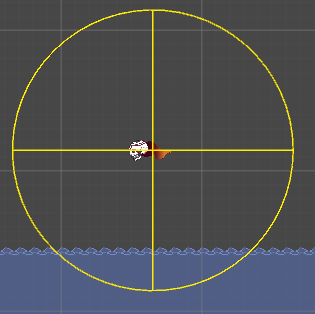
\includegraphics[width=0.4\textwidth]{03TrabajoRealizado/imagenes/EnemyRaycasting.png}
                    \caption{Ejemplo del área de acción del enemigo \textit{RedGhost}}
                    \label{fig:EnemyArea}
                \end{figure}
           
         \item \textbf{Cantidad de vida}: En el primer prototipo todos los enemigos
         eran derrotados por un único disparo, esto limitaba el factor de reto del
         juego al no ofrecer enemigos más resistentes al ataque del jugador. En el
         fin de ofrecer una nueva capa de complejidad a los enemigos se agrega a la
         clase \textit{Enemy} el atributo \textit{maxHealth} y \textit{healthAmount},
         estos atributos son los encargados de almacenar la máxima cantidad de vida
         que un enemigo puede tener y la vida actual de dicho enemigo (ver figura
         \ref{fig:EnemyAtributes}). La cantidad de
         vida sólo se actualiza cuando el enemigo es atacado por el jugador o cuando
         se reinicia el nivel. Para la actualización de la vida del enemigo se utiliza
         el comando \textit{Clamp} de la clase \textit{Math}, este comando permite
         especificar rangos con valores máximos y mínimos del resultado de operaciones,
         esto con la finalidad de que la vida actual del enemigo nunca sea cero y nunca
         sobrepase a su máximo de vida (ver figura \ref{fig:EnemyHealth}).
        
             \begin{figure}[h]
                    \centering
                    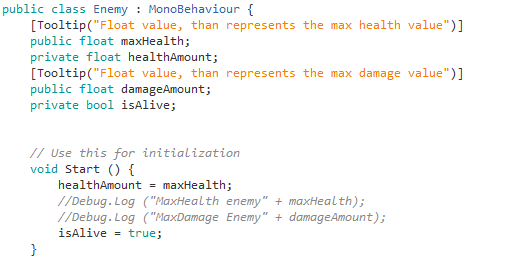
\includegraphics[width=0.6\textwidth]{03TrabajoRealizado/imagenes/EnemyClass.png}
                    \caption{Nuevos atributos para la clase \textit{Enemy}.}
                    \label{fig:EnemyAtributes}
            \end{figure}
            
            \begin{figure}[h]
                    \centering
                    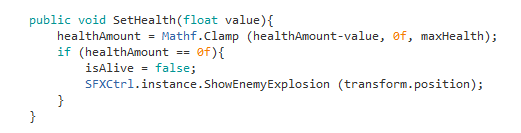
\includegraphics[width=0.6\textwidth]{03TrabajoRealizado/imagenes/EnemyClassMethodHealth.png}
                    \caption{Actualización de la cantidad de vida de la clase
                    \textit{Enemy}.}
                    \label{fig:EnemyHealth}
            \end{figure}
            
         \item \textbf{Cantidad de daño}: Al igual que con la cantidad de vida, los
         enemigos del primer prototipo infringen la misma cantidad de daño sin
         importar su tipo; por lo que para tener enemigos más y menos fuertes se agrega
         el atributo \textit{damageAmount}. Un enemigo puede infringir daño al jugador
         cada vez que toca al jugador o cuando dispara un ataque. Cada vez que un
         enemigo o un disparo enemigo choca con el jugador, el objeto enemigo manda
         a llamar el método \textit{SetHealth} del \textit{Player} y le envía como
         parámetro el valor de su atributo \textit{damageAmount}, seguido de un segundo 
         método
         de la clase \textit{Player} llamado \textit{EnemyNockBack}, este método es
         el encargado de la animación que indica que el jugador ha recibido daño (ver
         figura \ref{fig:PlayerGetsDamage}).
            
            \begin{figure}[h]
                \centering
                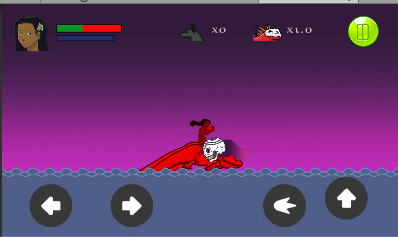
\includegraphics[width=0.4\textwidth]{03TrabajoRealizado/imagenes/EnemyRaycasting02.png}
                \caption{Ejecución de los métodos \textit{SetHealth} y \textit{EnemyNockBack} de la clase \textit{Player}, los cuales actualizan la cantidad de vida del jugador y muestran la animación de que el jugador ha recibido daño.}
                \label{fig:PlayerGetsDamage}
            \end{figure}
            
         \item \textbf{Girar horizontalmente}: En el primer prototipo el enemigo era
         incapaz de girar sus \textit{Sprite} y su ataque una vez que el jugador lo sobrepasaba como se ve en la figura \ref{fig:EnemyBack}. Utilizando la posición del enemigo y la posición del jugador dentro del área activa, el enemigo puede voltear su sprite y su ataque con base al valor de la distancia entre éste y el jugador:
         \begin{itemize}
             \item Si la posición del enemigo es mayor que las del jugador, el enemigo
             mantiene su orientación inicial.
             \item Si la posición del jugador es mayor que la del enemigo, el enemigo
             se voltea.
         \end{itemize}          

         Voltear un \textit{Sprite} no representa mayor problema en código; sin 
         embargo, el
         voltear un \textit{sprite} cuyo colisionador no es simétrico como el de 
         la figura
         \ref{fig:FixerCollider}. Esto puede representar un problema cuando se tiene
         que detectar colisiones, tal y como ocurre con los enemigos de tipo 
         \textit{RedGost} y
         \textit{PulpleGost}; para evitar alterar la detección de colisiones se 
         crea una nueva
         clase auxiliar llamada \textit{FixerCollider},  cuyo objetivo es ajustar 
         la posición
         del colisionador una vez que el personaje se gira como se puede observar en
         la figura \ref{fig:FixerCollider}.
        
         \begin{figure}[h]
                \centering
                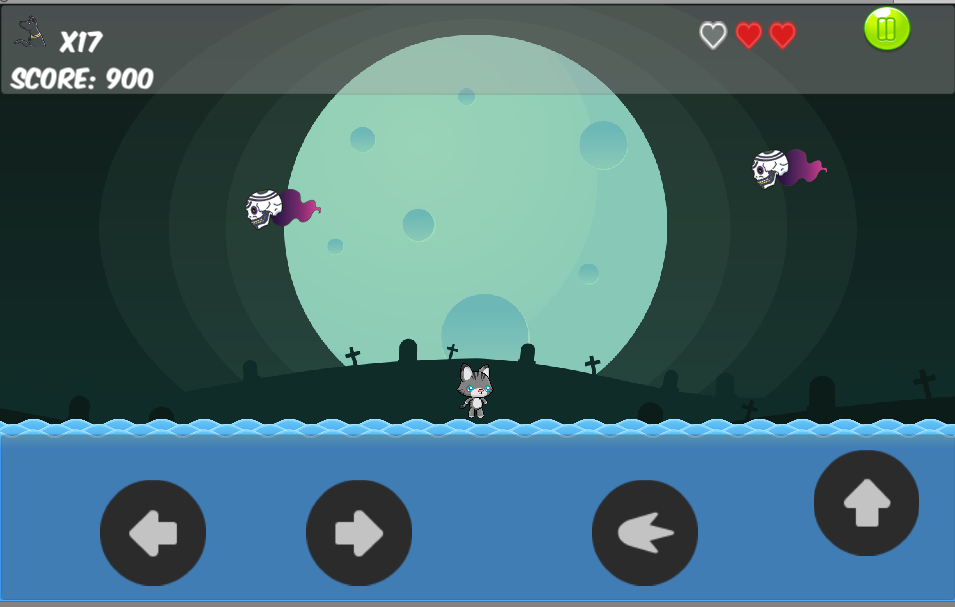
\includegraphics[width=0.4\textwidth]{03TrabajoRealizado/imagenes/voltearEnemigo01.png}
                \caption{En los primeros prototipos el enemigo es incapaz de girar su sprite y su ataque una vez que el jugador se coloca tras de éste.}
                \label{fig:EnemyBack}
        \end{figure}
        
        \begin{figure}[h]
              \centering
               \subfigure[ Ejemplo de un colisionador no simétrico respecto al \textit{sprite}.] {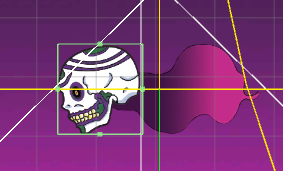
\includegraphics[width=0.3 \textwidth]{03TrabajoRealizado/imagenes/voltearEnemigo02.png}}
       
             \subfigure[Al girar el sprite de manera horizontal la posición del colisionador no se modifica]{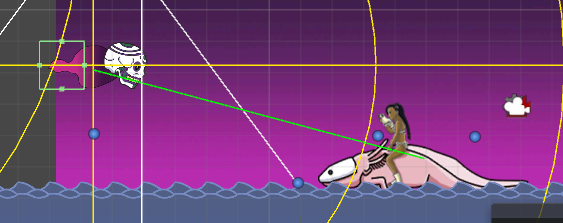
\includegraphics[width=0.3 \textwidth]{03TrabajoRealizado/imagenes/voltearEnemigo04.png}}
         
            \subfigure[Posición del colisionador modificada al emplear la clase \textit{FixerCollider}.] {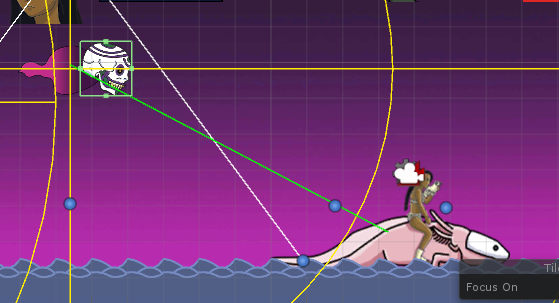
\includegraphics[width=0.3 \textwidth]{03TrabajoRealizado/imagenes/voltearEnemigo03.png}}
            
              \caption{Comportamiento del colisionador antes y después de la implementación de la clase \textit{FixerCollider}.}
              \label{fig:FixerCollider}
        \end{figure}
        
         \item \textbf{Trigger Collider}: En el primer prototipo el colisionador del
         enemigo tenía una configuración del tipo sólido lo que ocasionaba que cuando
         el enemigo chocaba con otro enemigo o con algún ataque enemigo este se
         estancara o fuera empujado por el objeto contra el que chocaba.
         Para corregir este comportamiento se configura el colisionador como uno de tipo
         trigger (ver figura \ref{fig:EnemyColliderTri}).  
            
            \begin{figure}[h]
                \centering
                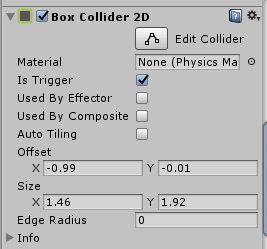
\includegraphics[width=0.3\textwidth]{03TrabajoRealizado/imagenes/Colisonador01.png}
                \caption{Configuración actual del colisionador de los enemigos.}
                \label{fig:EnemyColliderTri}
            \end{figure}    
        
         \item \textbf{Rigidbody2D}: Para evitar el comportamiento mencionado en el
         \textit{Trigger Collider} también fue necesario modificar la configuración
         del componente \textit{Rigidbody2D}, este componente pasa de estar en modo
         \textit{Dynamic} a modo \textit{Kinematic} lo que permite evitar que el objeto
         de juego reaccione conforme a las leyes físicas comunes.   
             
             \begin{figure}[h]
                \centering
                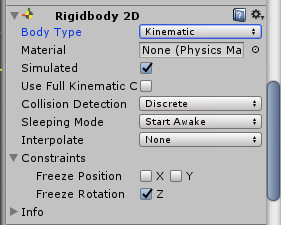
\includegraphics[width=0.3\textwidth]{03TrabajoRealizado/imagenes/Colisonador02.png}
                \caption{Configuración actual del componente \textit{Rigidbody2D} de
                los enemigos.}
                \label{fig:EnemyRigidBody}
            \end{figure}
    \end{itemize}

Para implementar cada uno de los patrones de movimiento de los enemigos es necesario
utilizar posiciones auxiliares que indiquen el límite del movimiento del personaje,
salvo en la clase Vulture ya que este explota al hacer contacto con el jugador. En la figura \ref{fig:JaguarCode} se puede observar el patrón de movimiento del enemigo de tipo jaguar expresado en código. Este comportamiento consiste en un movimiento recto horizontal de un punto A a un punto B y de regreso, haciendo una pausa en el movimiento cada vez que el jaguar ha alcanzado cualquiera de los puntos A o B (ver figura ).
\\
\par
            \begin{figure}[h]
                \centering
                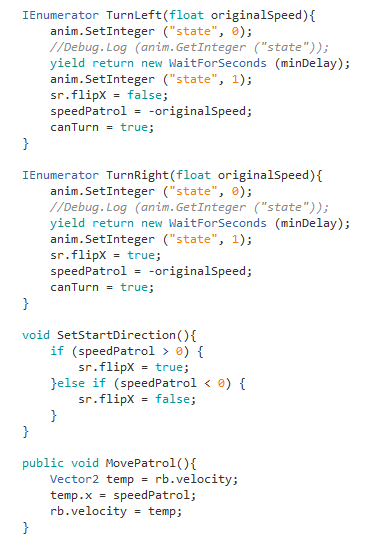
\includegraphics[width=0.3\textwidth]{03TrabajoRealizado/imagenes/PatronJaguar.png}
                \caption{Patrón de movimiento del enemigo tipo Jaguar expresado en
                código.}
                \label{fig:JaguarCode}
            \end{figure}
            
            \begin{figure}[h]
                \centering
                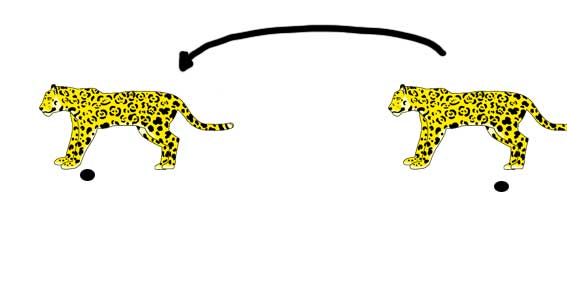
\includegraphics[width=0.3\textwidth]{03TrabajoRealizado/imagenes/saltoFelino.jpg}
                \caption{Patrón de movimiento del enemigo tipo Jaguar expresado en
                su comportamiento visual.}
                \label{fig:JaguarBeha}
            \end{figure}


Para resaltar la muerte de un enemigo se agrega un efecto especial de explosión
acompañado de un efecto de sonido para la explosión del personaje. Para esta
funcionalidad se implementa la clase \textit{SFXCtrl} y \textit{AudioCtrl} para 
manejar los efectos
de especiales y el sonido respectivamente, siendo estos los primeros controladores
en ser implementados.

\subsection{Implementando los enemigos jefes del juego}
Para la implementación de los enemigos jefes se reutilizan las configuraciones de los enemigos
normales referentes a las componentes \textit{Rigidbody2D} y \textit{Colisionador}, así como 
a la clase \textit{Enemy} para el manejo de vida y el uso de los efectos
de sonido y de explosiones para la muerte del jefe.
\\
\par
La lógica teórica tras los jefes del juego está inspirada por el jefe
\textit{Roxas} (ver figura \ref{fig:Roxas}) del juego \textit{Kingdom Hearts 2
Final Mix}. Dentro de \textit{Kingdom Hearts 2 Final Mix}, \textit{Roxas} es uno
de los jefes que requiere mayor habilidad de juego para ser derrotado, ya que a
diferencia del resto de los jefes de \textit{Kingdom Hearts 2 Final Mix}, el
patrón de ataque de \textit{Roxas} es totalmente aleatorio. Es decir, el jugador
puede saber en qué consiste cada uno de los ataques de este jefe, pero desconoce
el orden en el que estos serán ejecutados, salvo por algunos ataques que están
condicionados a una secuencia de ataque anterior.  Con los jefes del juego
\textit{Yolotl} sucede algo parecido, el jugador puede llegar a conocer lo tipos
de ataque que posee un jefe determinado pero la secuencia de ejecución de los
ataques está programada para que sea aleatoria, lo que puede generar experiencias
de juego muy sencillas o bastante retadoras para el jugador. El anterior
comportamiento se logra simulando una máquina de estados[referencia] 
con un arreglo de tipo booleano llamado \textit{whatCanDo}, en el cual solo un índice puede tener el
valor verdadero cada vez que se actualiza el estado y dependiendo del valor del
índice del valor verdadero será el ataque que ejecutará el enemigo. Después de
cada ataque el enemigo espera un tiempo determinado antes de asignar el siguiente
y ejecutarlo. Para ayudar al lector a comprender el funcionamiento de los jefes se
explica nuevamente usando como ejemplo al jefe \textit{Itzpapálotl} del nivel
cuatro. El jefe \textit{Iztpapálotl} cuenta con cuatro acciones:
    \begin{itemize}
        \item \textbf{\textit{WaitForAction:}} Espera un tiempo determinado y asigna
        un nuevo índice valor verdadero del arreglo de valores booleanos. Se activa
        si \textit{whatCanDo}[0] es verdadero.
        \item \textbf{\textit{shotFire}}: Dispara cuatro esferas de fuego que siguen
        al jugador y en caso de no chocar con este después de un tiempo se destruyen.
        Se activa si \textit{whatCanDo}[1] es verdadero.
        \item \textbf{\textit{useShell}}: Invoca un círculo de fuego que protege a
        \textit{Itzpapálotl} de cualquier daño, el escudo de fuego también puede
        infringir daño al jugador si hace contacto con éste. Se activa si
        \textit{whatCanDo}[2] es verdadero.
        \item \textbf{\textit{CreateButterflies}}: Invoca mariposas en tres puntos
        del campo, las mariposas también infringen daño al jugador y desaparecen
        después de un tiempo. Se activa si \textit{whatCanDo}[3] es verdadero.
    \end{itemize}
Al inicializarse el jefe \textit{Itzpapálotl whatCanDo}[0] es igual a cero. Por
lo que \textit{Itzpapálotl} ejecuta \textit{waitForAction}, al terminar la
ejecución de \textit{waitForAction}, \textit{whatCanDo}[0] es igual a falso y un nuevo
índice tiene ahora el valor verdadero. Supóngase ahora \textit{whatCanDo}[2] es
verdadero. \textit{Itzpapálotl} ejecuta \textit{useShell}, al terminar su
ejecución asigna \textit{whatCanDo}[2] como falso y asigna a \textit{whatCanDo}[0]
como verdadero. Nuevamente \textit{Itzpapálotl} espera unos segundos y actualiza
\textit{whatCanDo}. Por la naturaleza aleatoria de la actualización,
\textit{whatCanDo}[2] puede ser nuevamente verdadero o lo puede ser cualquier
otro índice exceptuando al 0 o a un número mayor que el índice máximo del
arreglo. En la figura se muestra la verificación de los valores de
\textit{whatCanDo} antes de la ejecución de cualquiera de los ataques que
tienen asignados. En la figura \ref{fig:EnemyMaquina} se muestra un ejemplo en
código de la maquina de estados del jefe \textit{Itzpapálotl}.
\\
\par
Por la forma en la que fue diseñado el comportamiento de la máquina de estados,
el nivel de dificultad que presente el jefe está dado en función de dos variables:
\textit{damageAmount} y \textit{timeBetweenAttacks}, correspondientes a la
cantidad de daño que el jefe puede infringir en el jugador y al tiempo que se
espera para actualizar los valores de \textit{waitForAction}. A mayor cantidad
de daño y menor tiempo de espera entre ataques, mayor será la dificultad para
derrotar al enemigo.

            \begin{figure}[h]
                \centering
                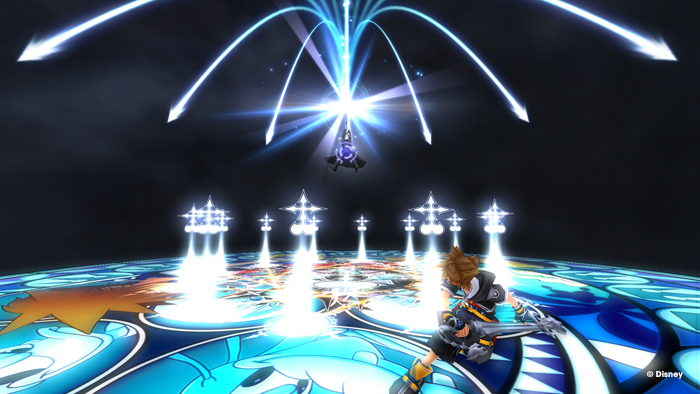
\includegraphics[width=0.5\textwidth]{03TrabajoRealizado/imagenes/RoxasBoss.jpg}
                \caption{\textit{Roxas} es el jefe más retador de \textit{Kingdom Hearts 2 Final Mix}. $ [Imagen] (2014)$ Recuperado de: \url{https://images.khinsider.com/2014\%20Uploads/05/Screenshots\%205-30/KHII_battle_03_EN\%20copy_1401446206.jpg}}
                \label{fig:Roxas}
            \end{figure}04R

            \begin{figure}[h]
                \centering
                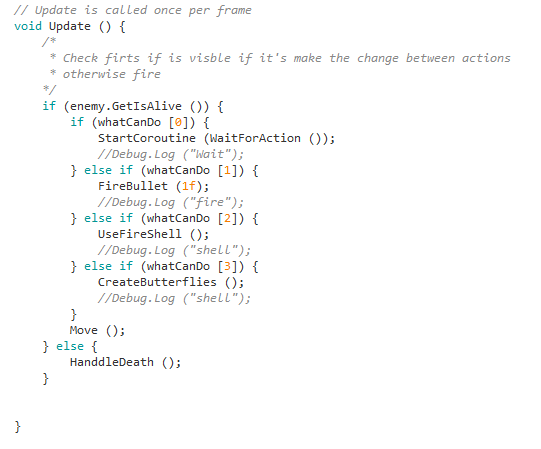
\includegraphics[width=0.5\textwidth]{03TrabajoRealizado/imagenes/ActualMaquinaJefe.png}
                \caption{Ejemplo de la máquina de estados del enemigo jefe.}
                \label{fig:EnemyMaquina}
            \end{figure}

\subsection{Implementando los ataques enemigos del juego}
Dentro del juego existen seis tipos de ataques enemigos:
    \begin{itemize}
        \item \textbf{Disparos con una trayectoria definida:} Este tipo de
        disparo sigue una trayectoria recta horizontal como se ve en la figura         
        \ref{fig:Enemyshot}.
        Para evitar la saturación de objetos dentro del juego, todos los disparos de
        este tipo se destruyen después de un tiempo. Para implementar este tipo de
        ataque se crea un \textit{GameObject} y se le agregan los siguientes
        componentes:
            \begin{itemize}
                \item \textbf{Collisionador:} El colisionador permite detectar si este
                ataque hace contacto con el \textit{Player} o con el suelo del nivel,
                en el primer caso se infringe daño al \textit{Player} y se destruye el
                \textit{GameObject}, en el segundo el \textit{GameObject} solo se
                destruye.
                \item \textbf{\textit{Rigidbody2D}}: El \textit{rigidbody2D} se
                configura
                con la opción \textit{kinematic} para evitar que el movimiento del
                disparo se vea afectado por la gravedad. Este componente permite en el
                código agregarle una velocidad al objeto.
                \item \textbf{\textit{DestryWithDelay}}: Componente creado por medio de
                la clase del mismo nombre, esta clase destruye al \textit{GameObject}
                que la contiene después de una cantidad determinada de tiempo.
                \item \textbf{\textit{EnemyBullet}}: Esta clase controla en la velocidad
                y dirección del movimiento del disparo, también tiene como atributo el
                daño que causa la bala y gestiona las colisiones del objeto.
            \end{itemize}
        Este tipo de disparo es empleado por los enemigos de tipo \textit{RedGost,
        Tepeyóllotl} y por \textit{Mictlantecuhtli}.
            
            \begin{figure}[h]
                \centering
                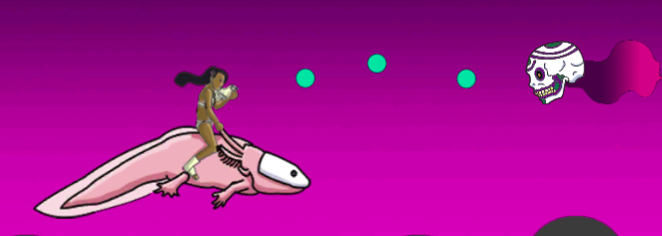
\includegraphics[width=0.5\textwidth]{03TrabajoRealizado/imagenes/disparoTrayectoria.png}
                \caption{Ejemplo de un disparo de una trayectoria definida.}
                \label{fig:Enemyshot}
            \end{figure}
            
        \item \textbf{Disparos que siguen al jugador}: Este tipo de disparo sigue un
        comportamiento y configuración parecida al anterior con la diferencia que en
        este tipo el disparo seguirá al jugador hasta impactarse contra éste o
        destruirse después de un tiempo si no colisiona contra el jugador. Este
        comportamiento requiere que el disparo tenga una referencia a la posición del
        jugador para moverse hacia él, en la figura \ref{fig:FollowedShot}se puede ver
        la implementación de disco comportamiento en código. Este ataque es utilizado
        por los enemigos de tipo \textit{Mictlantecuhtli}, \textit{Tepeyóllotl},
        \textit{Itzpapálotl, Xochitonal} y \textit{Tlazolteolt}. Para todos estos
        enemigos el disparo tiene el mismo efecto que es el de infringir
        daño en el jugador; sin embargo, en el tipo de \textit{Tlazolteolt} este tipo de
        disparo también puede disminuir la cantidad de \textit{Tonalli} del Player.
            
            \begin{figure}[h]
                \centering
                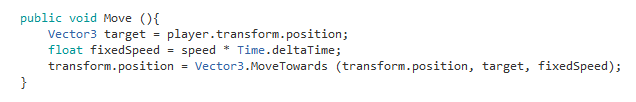
\includegraphics[width=0.5\textwidth]{03TrabajoRealizado/imagenes/disparoSigue.png}
                \caption{Implementación en código del comportamiento del disparo que sigue al jugador.}
                \label{fig:FollowedShot}
            \end{figure}        
        
        \item \textbf{Escudo de defensa que desaparece después de un tiempo}: Este
        ataque es efectuado por \textit{Itzpapálotl}. Al invocarse este escudo el
        enemigo no se ve afectado por los ataques del jugador. Este escudo no puede ser
        destruido y desaparece después de un tiempo que se invocó; este comportamiento
        se logra utilizando el método \textit{Invoke}, este método permite ejecutar
        métodos después de una cantidad de segundos; por lo que la desactivación se
        consigue mandando a llamar al método responsable de esto con \textit{Invoke}
        y asignando una cantidad determinada de segundos de espera.
        Inflige daño al jugador al hacer contacto con él.

        \item \textbf{Escudo de defensa que debe de ser destruido para desaparecer}:
        Ataque utilizado por \textit{Tlazolteolt}. Este escudo puede ser destruido
        por disparos del jugador y no desaparece al cabo de un tiempo. Al igual que el
        anterior protege al enemigo de los ataques del jugador e inflige daño si el
        jugador hace contacto con éste. Este tipo de escudo no cuenta con un método
        que lo desactive, en su lugar tiene una cantidad de vida determinada y que
        al llegar a cero, por efecto de los ataques del jugador, desaparece y reaparece
        hasta que el enemigo jefe lo vuelva a convocar.

        \item \textbf{Objetos que aparecen en posiciones cuya aparición tiene un tiempo
        de duración}: Este ataque es empleado por \textit{Itzpapálotl} y
        \textit{Mictlantecuhtli}. Cuando se activa provoca que se creen instancias del
        \textit{GameObject} que contiene la clase \textit{Butterfly}. Esta clase genera
        un movimiento vertical ascendente e inflige daño al jugador al hacer contacto
        con esta. La creación de estos \textit{GameObjects} se mantiene activa por un
        periodo de tiempo y después desactiva.Este funcionamiento se logra de una
        manera similar al comportamiento del escudo de defensa que desaparece después
        de un tiempo utilizando el método \textit{Invoke}. En la figura se puede
        observar la implementación en código de este tipo de ataque.  

        \item \textbf{Objetos que aparecen en posiciones de manera periódica}: Este
        ataque genera una lluvia de huesos o de piedras que le infringen daño al
        jugador una vez hacen contacto con este de lo contrario se destruyen al hacer
        contacto con el suelo. Para la creación de los objetos se utiliza el método
        \textit{Invoke} el cual controla la cantidad de \textit{GameObject} que se
        crean. Este ataque es utilizado por \textit{Mictlantecuhtli} y
        \textit{Tepeyóllotl}.
    \end{itemize}
 
\subsection{Implementando los obstáculos}
Una de las características de un juego de plataformas es la existencia de diferentes
obstáculos que el jugador debe de superar por medio de saltos\cite{Ref_JuegoDisenio}.
En \textit{Yolotl} se diseñaron e implementaron diferentes tipos de obstáculos
para ofrecer una variedad de retos al jugador, a continuación, se describe cada
uno de ellos y cómo fue que fueron implementados en el juego:
    \begin{itemize}
        \item \textbf{Plataforma que se mueve:} Es uno de los elementos más comunes de
        los juegos de plataforma, este   obstáculo consiste en una superficie de que
        se mueve de una posición a otra, ver figura \ref{fig:MovingPlatform}. dentro
        del juego se creó la clase \textit{MovingPlatform} para este tipo de obstáculo.
        \textit{MovingPlatform} tiene por atributos las posiciones a las que se moverá,
        velocidad a la que se moverá. Para su movimiento la clase hace uso de cuatro
        vectores de posiciones \textit{pos01, pos02, startPos} y \textit{nextPos}.
        \textit{Pos01} y \textit{pos02} son las posiciones límite que alcanzará la
        plataforma, \textit{startPos} es la posición hacia la que la plataforma inicie
        su movimiento inicial y \textit{nextPos} es la siguiente posición a la que se
        ira la plataforma una vez que haya alcanzado un límite. Manejar el
        comportamiento de las plataformas móviles con este sistema de posiciones
        permite que la plataforma pueda tener movimiento horizontal, vertical o diagonal
        sin la necesidad de reescribir código. Al igual que con los enemigos las
        plataformas de este tipo tienen un radio de área activa para evitar que su
        comportamiento se ejecute si no están visibles al jugador. Asignar el movimiento
        de la plataforma no es suficiente para su correcto funcionamiento, ya que
        cuando el movimiento de la plataforma es horizontal, ésta se desplaza sin el
        personaje ya que por sí misma no es capaz de asignarle un movimiento al jugador,
        por tal motivo fue necesario crear una nueva etiqueta para las plataformas
        llamada \textit{Platform} y asignar dos nuevos parámetros en las colisiones
        al jugador
        una para cuando entra en contacto con el colisionador de la plataforma y otra
        cuando sale. Cuando el jugador entra en contacto con el colisionador de la
        plataforma se le asigna un parentesco con la posición de la plataforma, lo
        que le permite seguir el movimiento de la plataforma, este parentesco se
        rompe cuando el jugador sale de la plataforma, en la figura
        \ref{fig:MovingPlatformCol} se puede ver esto en código. Adicionalmente,
        se utilizó el comando \textit{OnDrawGizmos} para dibujar la trayectoria de la
        plataforma a fin de facilitar la configuración de las plataformas móviles en la
        construcción de los niveles, ver figura \ref{fig:MovingPlatformWay}.
            
            \begin{figure}[h]
                \centering
                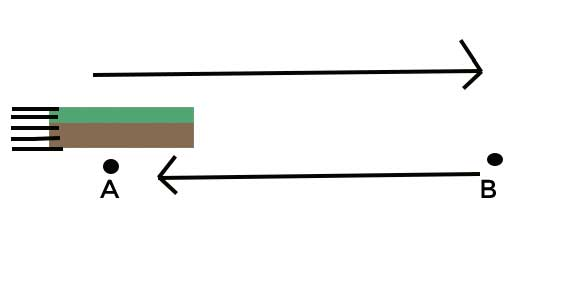
\includegraphics[width=0.5\textwidth]{03TrabajoRealizado/imagenes/plataformaMovil.jpg}
                \caption{Comportamiento de la plataforma que se mueve de manera visual.}
                \label{fig:MovingPlatform}
            \end{figure}
            
            \begin{figure}[h]
                \centering
                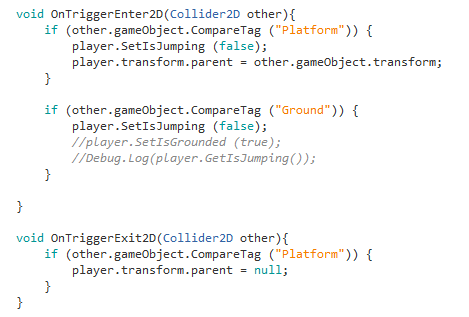
\includegraphics[width=0.5\textwidth]{03TrabajoRealizado/imagenes/plataformaColisiones.png}
                \caption{Gestión de la respuesta ante diferentes colisiones para
                garantizar el comportamiento de una plataforma que se mueve de manera
                horizontal.}
                \label{fig:MovingPlatformCol}
            \end{figure}
            
            \begin{figure}[h]
                \centering
                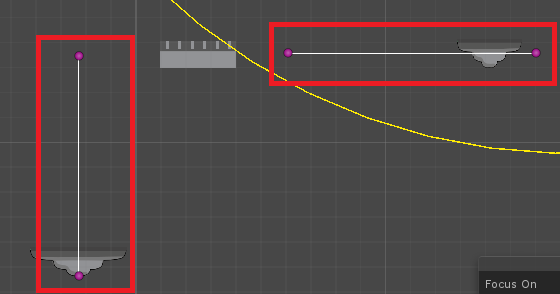
\includegraphics[width=0.5\textwidth]{03TrabajoRealizado/imagenes/plataformaConfig.png}
                \caption{Uso del método \textit{OnDrawGizmos} para visualizar la
                trayectoria de una plataforma que se mueve.}
                \label{fig:MovingPlatformWay}
            \end{figure}

        \item \textbf{Plataforma que cae}: Este tipo de plataforma se cae después de
        que el jugador se posiciona sobre ella. Para evitar que la plataforma caiga
        instantáneamente una vez que el jugador ha caído sobre ella, un tiempo de
        retraso se le asigna a la caída.

        \item \textbf{Plataforma con más de dos posiciones de control}: esta plataforma
        puede seguir patrones complejos movimiento como círculos, rectángulos o
        cuadrados. Su funcionamiento es similar a la plataforma que se mueve con la
        diferencia de que soporta más de dos posiciones de control; para esto se vale
        de un arreglo de posiciones en donde el atributo de \textit{nextPos} recorre
        todo el arreglo de posiciones y al llegar al último elemento del arreglo se
        le asigna el valor del primer elemento reiniciando el recorrido, ver figura .

        \item \textbf{Viento}: Ese obstáculo crea una corriente de viento que empuja
        al jugador hacia el vacío, ver figura . Para crear este obstáculo se crean
        tres clases: \textit{PushingObstacle}, \textit{WindCreator} y
        \textit{WindHelper}. La primera controla el movimiento del viento a crear.
        La segunda crea el viento por periodos de tiempo dejando un tiempo de
        inactividad para que el jugador pueda pasar y la tercera activa al creador
        de viento cuando el jugador entra en el área activa del obstáculo, cada clase
        está instanciada en un \textit{GameObject} diferente. En un principio solo
        existían las clases \textit{PushingObstacle} y \textit{WindCreator}, lo que
        provoca que el creador de viento cree viento aun cuando el obstáculo no es
        visible para el jugador; esto ocasiona la creación de muchos
        \textit{GameObjects} innecesarios para el viento, por tal motivo se crea la
        clase \textit{WindHelper} para controlar la activación del
        creador de viento.  Para definir los periodos de creación de viento y de pausa
        de viento es necesario probar diferentes valores para asignar los tiempos de
        creación y de pausa del viento. Luego de varias pruebas se definen los
        siguientes tres valores: 4 para el tiempo activo de creación, 8 para el tiempo
        de pausa de viento y 0.4 para la pausa entre creación de instancias de viento.

        \item \textbf{Estalagmitas}: Este obstáculo se cae e inflige daño en el
        jugador cuando éste pasa por debajo del obstáculo, ver figura .  Para
        implementar este obstáculo se crean dos clases: \textit{Stalagmite} y
        \textit{StalagmiteCtrl}. La primera clase gestiona la caída del objeto y el
        daño que le infringe al jugador si choca con este o la destrucción del objeto
        en caso de que choque con el suelo. La segunda clase se encarga de indicarle
        a la clase \textit{Stalagmite} que el jugador va a pasar bajo de ella para que
        inicie su caída. En la figura \ref{fig:StalagmiteConf} se puede ver la
        configuración de ambos objetos dentro de un nivel.
        
            \begin{figure}[h]
                \centering
                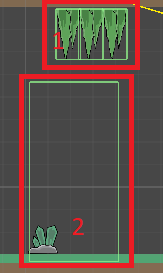
\includegraphics[width=0.3\textwidth]{03TrabajoRealizado/imagenes/StalagmiteConfig.png}
                \caption{Configuración de los diferentes \textit{GameObjects} que
                conforman el obstáculo estalagmita.}
                \label{fig:StalagmiteConf}
            \end{figure}
        
        \item \textbf{Obstáculo que hace daño}: este obstáculo infringe daño al jugador
        cuando éste hace contacto con él y no puede ser destruido por el mismo. Este
        tipo de obstáculo se puede encontrar en el segundo nivel en la etapa de
        plataforma. Para su implementación se crea la clase \textit{DamageObstacle} y 
        esta
        gestiona el daño que infringe el obstáculo pudiendo generar obstáculos que
        causen más o menos daños que otros.

        \item \textbf{Xólotl en su forma Colibrí}: Este obstáculo tiene un
        comportamiento parecido a la plataforma con más de dos posiciones de
        control anteriormente descrita, con la diferencia de que su movimiento
        describe una línea y no un circuito cerrado; por otro lado, al morir el
        jugador este obstáculo regresa a su posición inicial. Este obstáculo aparece
        únicamente en el nivel 6, donde el jugador deberá cruzar distintos segmentos
        del mapa sobre este obstáculo y tendrá que vencer a los enemigos que vayan
        apareciendo para avanzar, ver figura .
    \end{itemize}

\subsection{Implementando los ítems y los objetos coleccionables}
Las últimas clases actoras en ser implementadas fueron los ítems, los objetos
coleccionables y los puntos de guardado, ya que en el caso de los ítems y los
puntos de guardado se necesitaba que el jugador sufriera daño, gastara
\textit{tonalli} o muriera ya fuera a causa de enemigos u obstáculos.
\\
\par
Dentro del juego existen dos tipos de ítems: Los que recuperan cantidad de vida y
los que recuperan cantidad de tonalli. Ambos tienen un funcionamiento similar: como
atributos sus respectivas clases tienen una cantidad de lo que van a restaurar
(sea \textit{tonalli} o vitalidad), al hacer contacto con el jugador le incrementan
dicho atributo en la cantidad que tienen asignada y se destruyen mostrando un
efecto de brillos y un efecto de sonido.
\\
\par
En lo que se refiere a los objetos coleccionables dentro del juego se crea la
clase CollectableObjects, clase encargada de destruir los objetos coleccionables
una vez que el jugador los ha tocado, dejando la tarea de actualizar el marcador
al jugador. Para poder lograr la actualización del atributo \textit{score} del
\textit{Player} se asignaron etiquetas para los objetos coleccionables y dependiendo
de dichas etiquetas se gestiona la actualización de los marcadores, esto debido a que
la función de los objetos coleccionables depende directamente del nivel en el que
se encuentre el jugador; por ejemplo, para los perros que aparecen en el segundo
nivel, hacer contacto con uno de ellos no solo actualiza el marcador sino también
incrementa el poder que tendrá el Jefe de este nivel, por lo tanto
la actualización visual del marcador deberá incluir cuantos perros se han tocado
y en cuanto se ha incrementado el poder del jefe(ver figura
\ref{fig:CollectableObjects}); mientras que en el nivel 4, los coleccionables
son llaves y su función es la de desbloquear la transición al siguiente nivel
solo si se han juntado todas las llaves; visualmente esta actualización solo
requiere de la actualización de un elemento en pantalla (ver figura 
\ref{fig:CollectableObjects}). Para solucionar esto se crearon dos etiquetas 
para cada tipo de coleccionable: \textit{CollectableDog} y 
\textit{CollectableKey}.  Dejando al gestor de colisiones de la clase 
\textit{Player} verificar por medio de la etiqueta de qué tipo de coleccionable 
se trata e invoca al controlador de la interfaz gráfica de los marcadores del 
juego o \textit{HUB}.
            
            \begin{figure}[h]
              \centering
               \subfigure[El marcador referente a los perros se encuentra en cero, ya
               que el jugador no ha tocado ninguno de estos.] {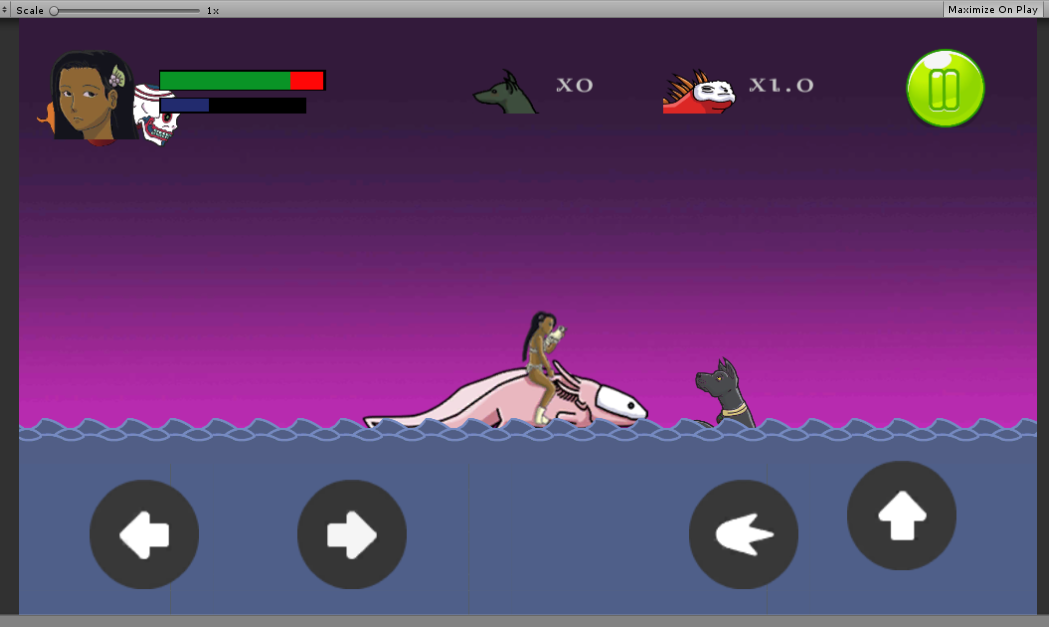
\includegraphics[width=0.3 \textwidth]{03TrabajoRealizado/imagenes/InterfazJuego06.png}}
       
             \subfigure[Al tocar un perro el marcador referente al conteo de ellos se actualiza junto al del poder del jefe.]{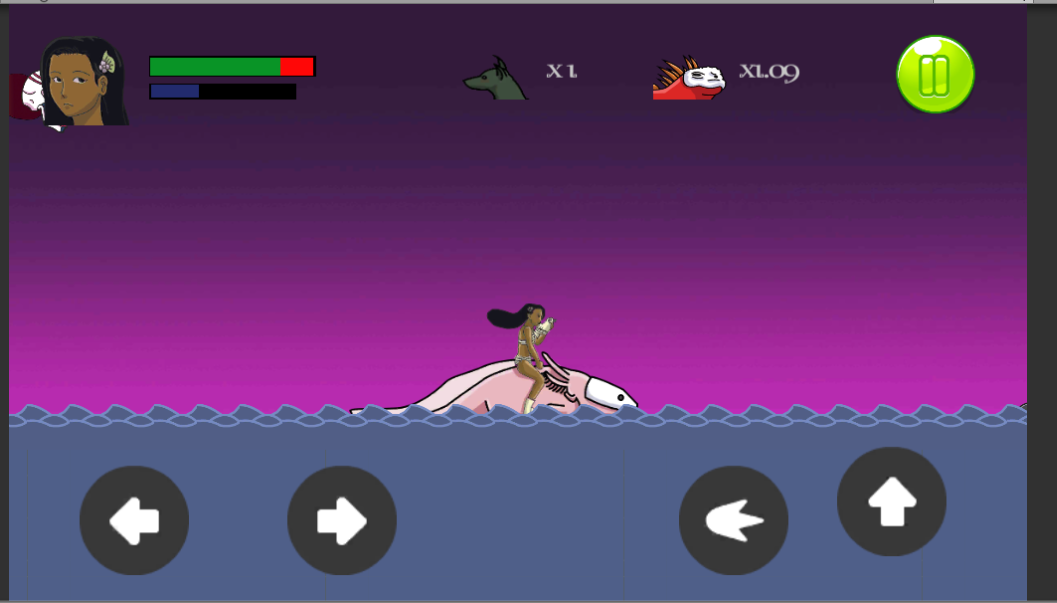
\includegraphics[width=0.3 \textwidth]{03TrabajoRealizado/imagenes/InterfazJuego07.png}}
            
              \caption{Interacción entre el jugador y los objetos coleccionables del nivel.}
              \label{fig:CollectableObjects}
        \end{figure}

\subsection{Implementación de los puntos de guardado}
Los puntos de guardado o \textit{checkpoints} son los actores encargados de
hacer aparecer al jugador en una posición del nivel una vez que éste haya muerto,
evitando que el jugador pierda su progreso dentro del nivel. Un
\textit{checkpoint} se activa cuando el jugador hace contacto con éste. La
funcionalidad de este actor está dada por la clase \textit{CheckPoint}, esta clase
tiene como atributos(ver figura \ref{fig:CheckAtri}):

\begin{itemize}
    \item \textit{\textbf{isActive}}: Atributo booleano. Cuando es verdadero indica
    que el jugador  ha pasado por el checkpoint. Solo puede haber un único checkpoint
    activo.
    \item \textit{\textbf{CheckPointsList}}: Arreglo de GameObjects que instancian
    la clase CheckPoint.
\end{itemize}

Cuando el jugador entra en contacto con el \textit{checkPoint}, éste manda a
llamar el método \textit{ActivateCheckPoint}, este método toma todos los
elementos que hay en  \textit{CheckPointsList} y vuelve su atributo
\textit{isActive} falso, después vuelve verdadero el atributo \textit{isActive}
del \textit{checkPoint} que fue tocado por el jugador. Cuando el jugador muere
se manda a llamar el  método \textit{GetActivePosition}, este método busca el
\textit{checkPoint} activo y revive al jugador en esa posición. En la figura
\ref{fig:CheckMethod} se muestran los métodos de esta clase.

Existen dos tipos de \textit{checkPoints}:
    \begin{itemize}
        \item \textbf{\textit{CheckPoint} vacío}: este \textit{checkPoint} no 
        tiene ningún
        \textit{sprite} asignado y se encuentra al inicio del nivel. Está activo 
        por defecto
        y si el jugador muere sin antes tocar algún otro \textit{checkPoint}, la
        posición de este \textit{checkPoint} es donde aparecerá al revivir.
        \item \textbf{\textit{CheckPoint} normal}: Este \textit{checkPoint} tiene un
        búho como \textit{sprite} y una animación para cuando el jugador interactúa con
        él.
    \end{itemize}
    
\begin{figure}[h]
                \centering
                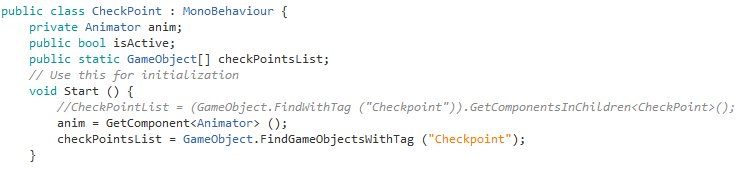
\includegraphics[width=0.3\textwidth]{03TrabajoRealizado/imagenes/checkpoint.png}
                \caption{Atributos de la clase \textit{CheckPoint}}
                \label{fig:CheckAtri}    
\end{figure}

\begin{figure}[h]
                \centering
                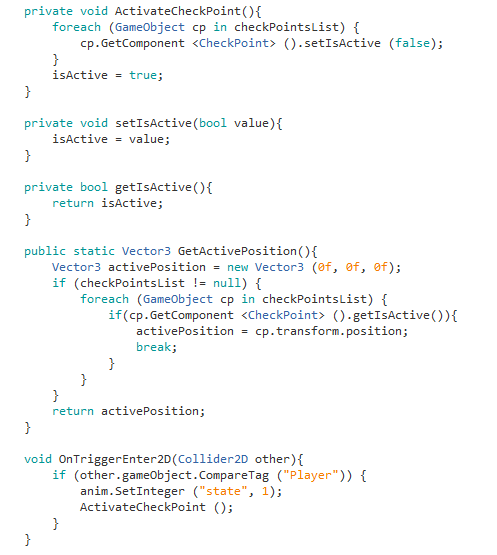
\includegraphics[width=0.3\textwidth]{03TrabajoRealizado/imagenes/checkpointmethods.png}
                \caption{Métodos de la clase \textit{CheckPoint}}
                \label{fig:CheckMethod}    
\end{figure}

\subsection{Cierre del sprint}
Al término de este \textit{sprint} se cuenta con todos los \textit{Assets} de
los actores organizados en diferentes carpetas como \textit{Player, Obstacles, Enemies},
etc. Este \textit{sprint} se cierra con éxito y deja todos los elementos listos
para la construcción de las clases controladoras.
